\subsection{Paraview \label{app:paraview}}

\subsubsection*{Installation procedure}

If you have Ubuntu, type the following in a terminal and follow the instructions. 
\begin{verbatim}
sudo apt-get install paraview
\end{verbatim}
Upon completion, type 'paraview' followed by Enter in the terminal and your screen should look similar to Screen Capture 1.

If you run Windows or MacOS\footnote{You could also use Home Brew 
\url{https://formulae.brew.sh/cask/paraview}}, go to \url{www.paraview.org}. 
Click on 'download'. The website automatically detects your 
OS\footnote{\url{https://en.wikipedia.org/wiki/Operating_system}}. 
Download the latest version(.exe for Windows, .dmg for Apple), and install it on your computer. 
Find the icon on your computer, double click on it and your screen should look similar to Screen Capture 1.

\begin{center}
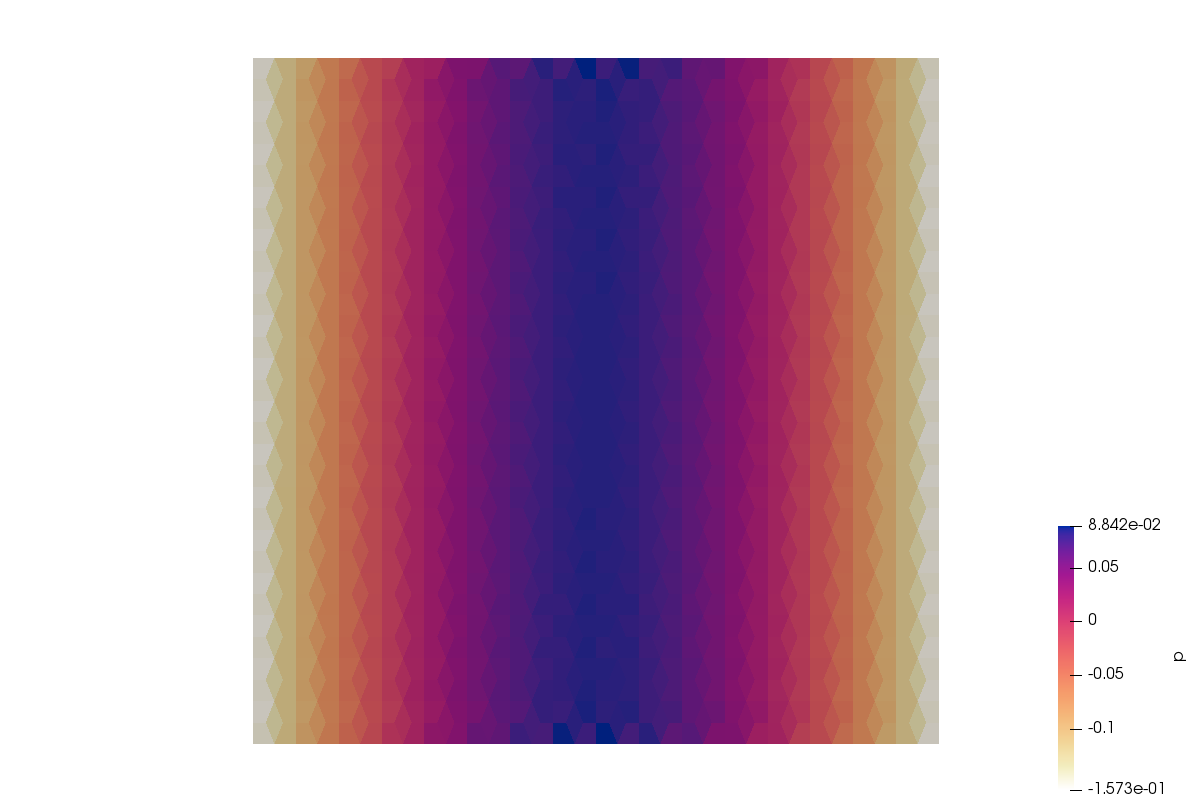
\includegraphics[width=10cm]{images/paraview/p1}\\
{\captionfont Screen Capture 1.}
\end{center}

%---------------------------------------
\subsubsection*{Opening a file}

Press Ctrl+O on your keyboard or click File$>$Open$>$ and the following window should appear after you press the 
green button Apply:

\begin{center}
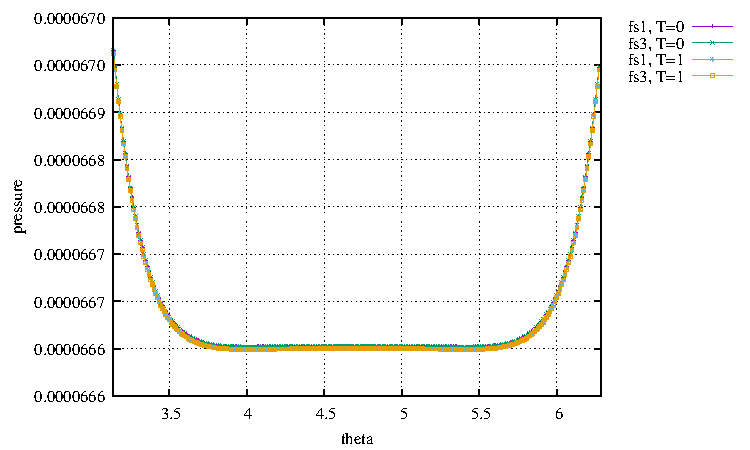
\includegraphics[width=10cm]{images/paraview/p2}\\
{\captionfont Left click of the mouse allows you to move the domain in the plotting area, 
Right click allows you to zoom in and out.}
\end{center}

Select the .vtu file you wish to import in the session or a whole list of them. 
Your Paraview session should then look like this:
 
\begin{center}
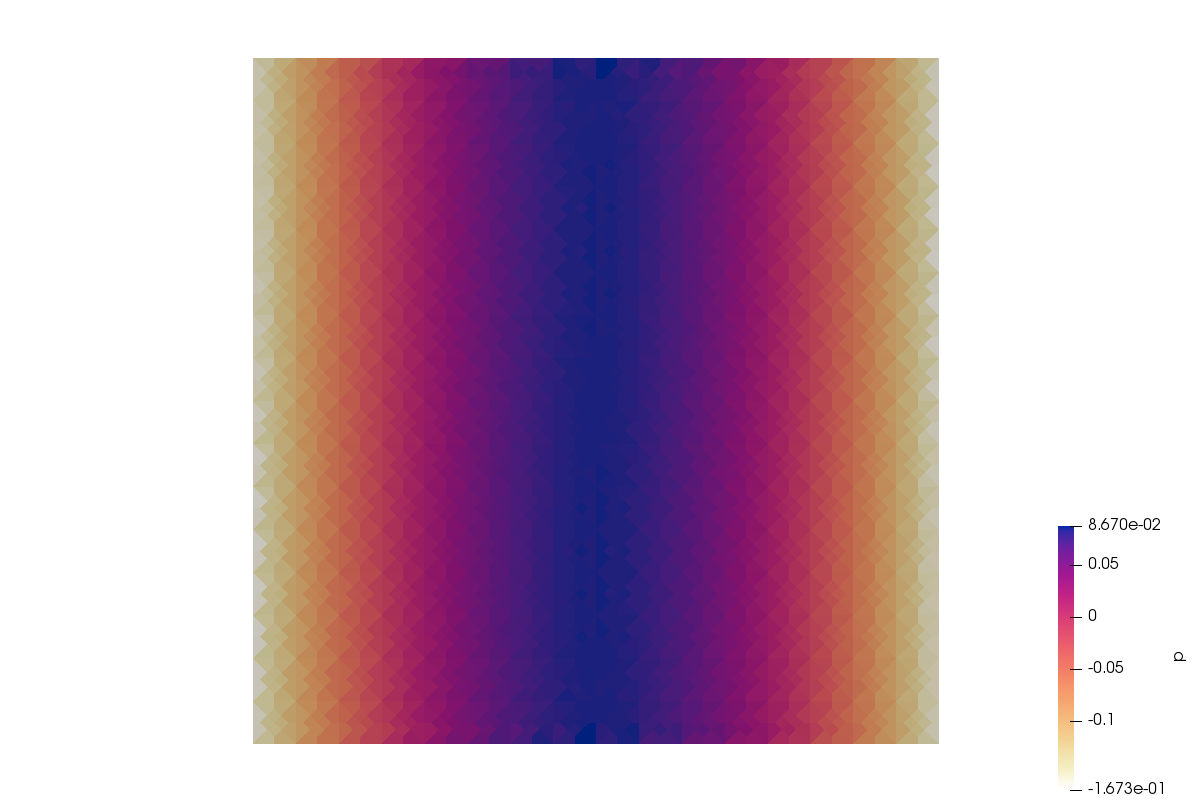
\includegraphics[width=10cm]{images/paraview/p3}\\
{\captionfont 1: click on this icon to change the background colour to white;\\
2: click this icon for plotting vector field arrows and follow instructions below;\\
3: click this icon for isocontours and follow the intructions below.\\}
\end{center}


\begin{center}
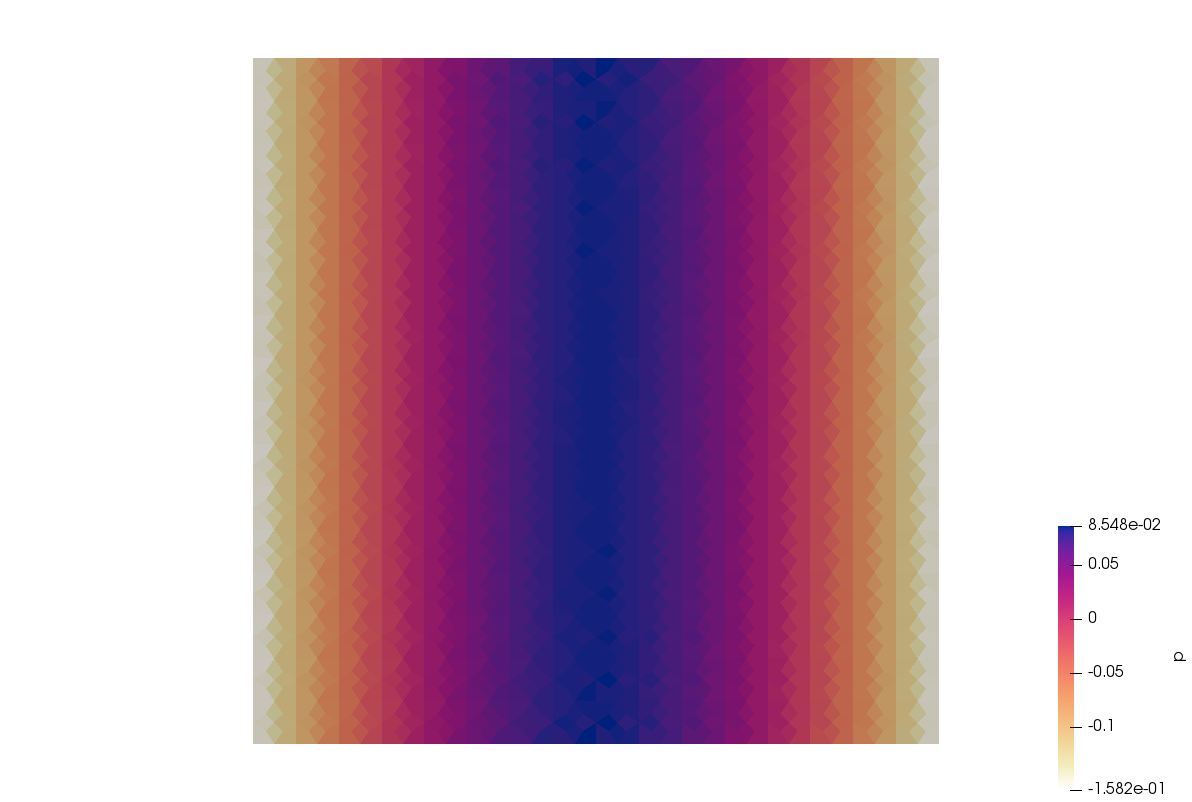
\includegraphics[width=10cm]{images/paraview/p4}\\
{\captionfont 4: click on this menu to select the field you wish to plot;\\
5: click on this menu and select Surface With Edges to see the mesh;\\
6: click on this icon to remove the red-yellow-green axis in the plotting area.\\}
\end{center}



%--------------------------------------
\subsubsection*{Colours and log scale}

I have loaded the .vtu file, chosen a white background, zoomed in, selected the temperature field, so that 
my screen looks now like this (I have also moved the colour bar):

\begin{center}
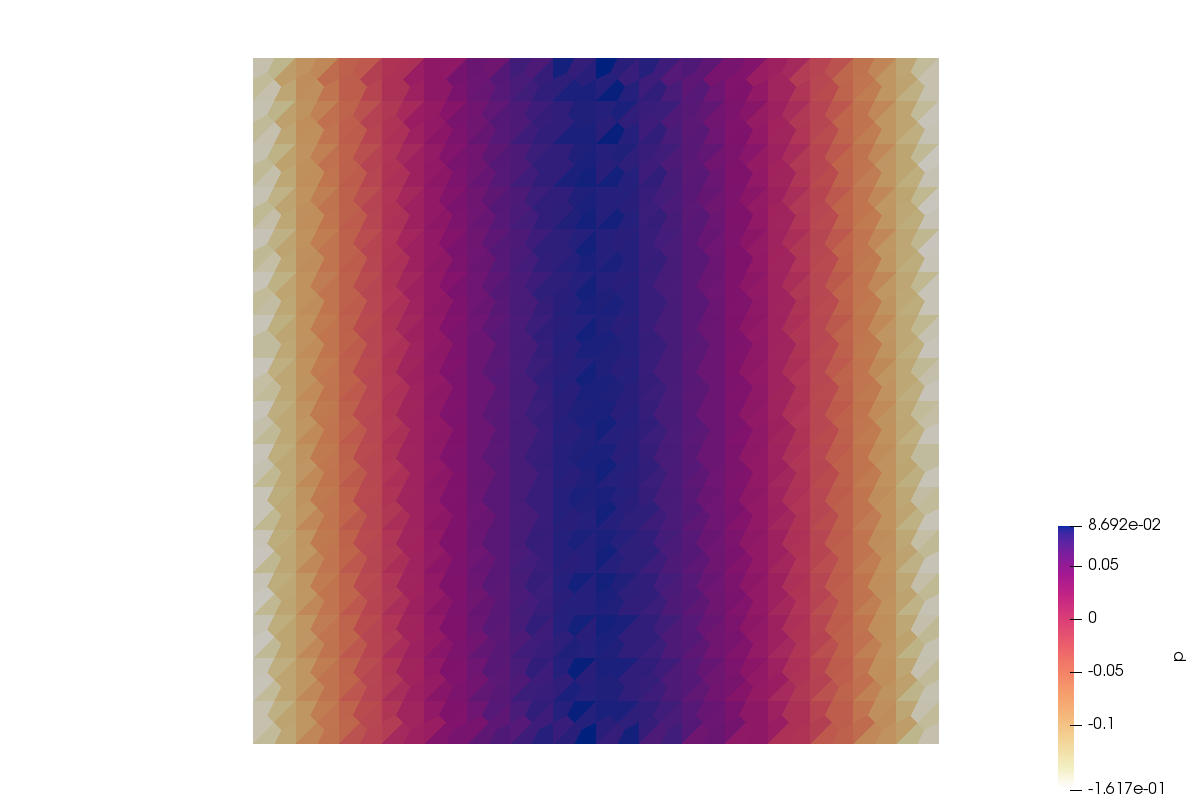
\includegraphics[width=10cm]{images/paraview/p5}\\
{\captionfont 7: change the range of the variable; \\
8: change the colour scale; \\
9: change the number of colours inside the scale; \\
10: switch on logarithmic scale.}
\end{center}

When it comes to choosing colours, please see: 
\textcite{crsh20} and  \textcite{vacp22}.


\begin{center}
\includegraphics[width=10cm]{images/paraview/p11}\\
{\captionfont If you find that the circled area is missing on your screen, 
go to View and click on Color Map Editor.}
\end{center}

\todo[inline]{add how to add color scales}

%--------------------------------------
\subsubsection*{Isocontours}

Having clicked on the icon numbered 3 in the panels above, 
your screen should look like this:

\begin{center}
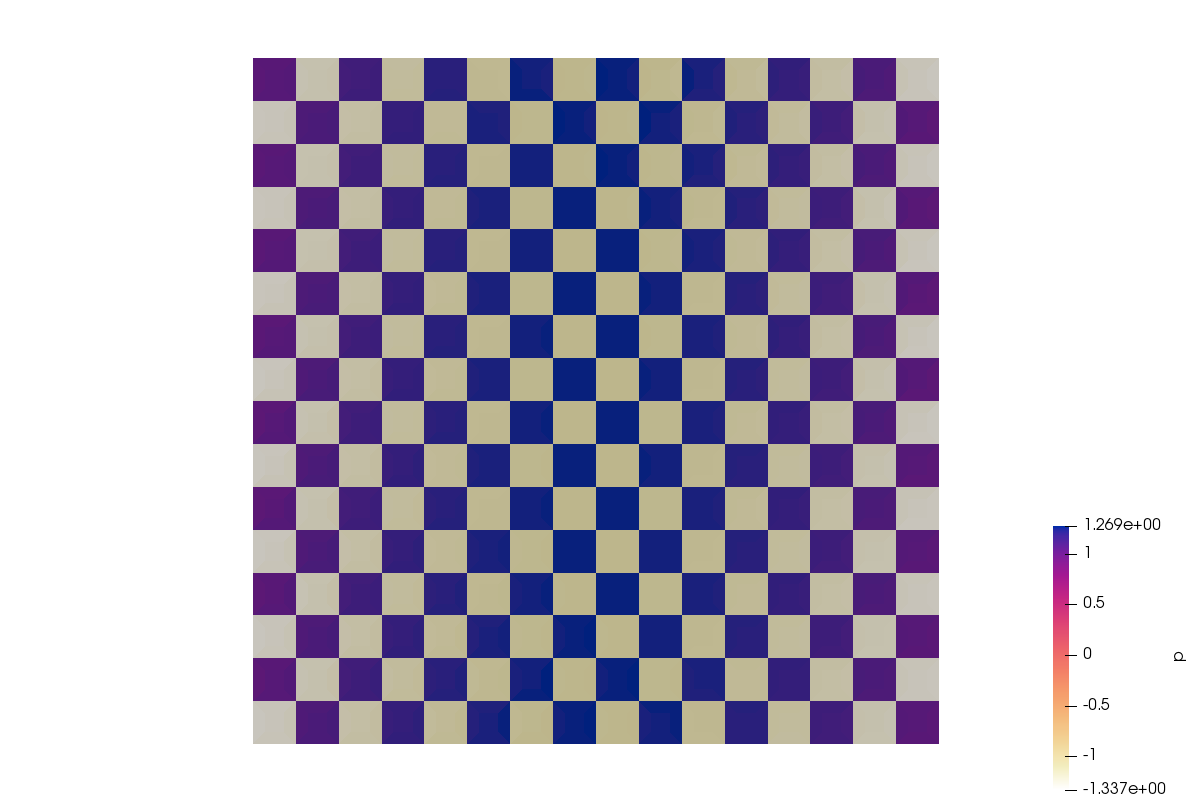
\includegraphics[width=10cm]{images/paraview/p7}\\
{\captionfont 11: value of the isocontour; \\
12: add or remove an isocontour;\\
13: toggle the background grey square and the isocontours on/off by clicking on their respective eye.}
\end{center}


\begin{center}
\includegraphics[width=8cm]{images/paraview/p8}
\includegraphics[width=8cm]{images/paraview/p9}\\
{\captionfont Left: If you want automatically generated isocontours, 
remove the existing one and click on 20. A small window opens: 
fill the min/max/number values and click OK.
Right: Having obtained these isocontours you can change the colour of the lines 
by clicking on 19.}
\end{center}

%---------------------------------------------------------------
\subsubsection*{Vector field arrows}

\begin{center}
\includegraphics[width=10cm]{images/paraview/p10}\\
{\captionfont In order to obtain such arrows, make sure that you go through points 14 and 15.\\ 
Then click on the icon 16. In order to change the scale of the arrows change the value in 17.}
\end{center}


%----------------------------------
\subsubsection*{Exporting to png}

File$>$Save Screenshot. Click OK on the first panel. Enter the name of the file you have chosen and click OK.   

%----------------------------------
\subsubsection*{Exporting line data}

Filters $>$ Data Analysis $>$ Plot Over Line.  

\begin{center}
\includegraphics[width=10cm]{images/paraview/p13}\\
{\captionfont You can change the coordinates of the beginning and the end of the line.} 
\end{center}

%---------------------------------------
\subsubsection*{Getting rid of 'Apply'}

It can be annoying to have to press Apply all the time so if you wish to bypass it, got to Edit $>$ Settings, and 
tick the 'Auto Apply' box in the window that appears.

%---------------------------------------
\subsubsection*{Multiple vtu files at once}

\begin{center}
\includegraphics[width=10cm]{images/paraview/p14}\\
{\captionfont You can load multiple vtu files or the same one multiple times and move each where you want it.} 
\end{center}

%---------------------------------------
\subsubsection*{Warp by scalar}

\begin{center}
\includegraphics[width=6cm]{images/paraview/p15a}
\includegraphics[width=6cm]{images/paraview/p15b}\\
{\captionfont Filters $>$ Alphabetical $>$ Warp By Scalar} 
\end{center}






